\documentclass{beamer}
%\documentclass[notes]{beamer}

\usepackage{inputenc}
\usepackage{graphicx}

\usetheme{Warsaw}

\title{A Case for an SC-Preserving Compiler}
\subtitle{Daniel Marino, Abhayendra Singh, Todd Millstein, Madanlal Musuvathi, Satish Naranasamy}

\author{Presented by \\ Akshay Gopalakrishnan}

\institute{McGill University}

\begin{document}
    
    \begin{frame}

        \titlepage
    
    \end{frame}

    %Introduction 
    \begin{frame}{Introduction}

        \begin{itemize}
            \item Relaxed memory models.
            \item Program transformations for high performance.
            \item Many of them are SC-Preserving.
            \item Non-SC preserving transformations can be broadly attributed to reorderings.
            \item A speculation based language construct to perform load-store reorderings when SC-Preserving. 
            \item Much of the performance is retained. 
        \end{itemize}

    \end{frame}

    \notes{It is important to note that some of the findings (empirical or otherwise) may be obsolete as this is a work done quite some years ago.
    To add, the observations by the authors were on the LLVM passes, which to be honest has been evolving rapidly.
    It might be the case that their conclusions about performance might be completely obsolete. 
    However, their findings which cleanly categorize program transformations as SC or Non-SC preserving help a lot.}

    %Primer to Memory Models
    \begin{frame}{Memory Consistency Model - Sequential Consistency}

        Memory consistency model describes what values a read can have in a concurrent execution.
        \\        
        \center \textit{Sequential consistency guarantees that the read values of any concurrent execution of a program can always be justified by an execution of the same program in a uniprocessor (interleaving semantics).} 

    \end{frame}

    %Example of Weak memory behaviors
    \begin{frame}{The need for Relaxed Memory Model}

        Sequential consistency is:
        \begin{itemize}
            \item Too strict which prevents much of the performance H/W provides.
            \item Too strict to do common compiler optimizations responsible for a lot of performance benefits (eg: Common Sub-expression elimination)
        \end{itemize}

        Relaxed memory models:
        \begin{itemize}
            \item Describe pretty well what freedom hardware provides for reads (Store/Load buffers, Speculation, (Non)Multicopy Atomicity, etc). 
            \item Allows a large class of compiler optimizations responsible for performance (high level languages).  
            \item Giving low level constructs to provide fine grained concurrency (eg: Store-Load fence, MFence, Lwsync, etc).
        \end{itemize}

    \end{frame}

    \begin{frame}{Example of Non-SC Preserving Transformation}

        \begin{figure}
            \makebox[\textwidth][c]{
                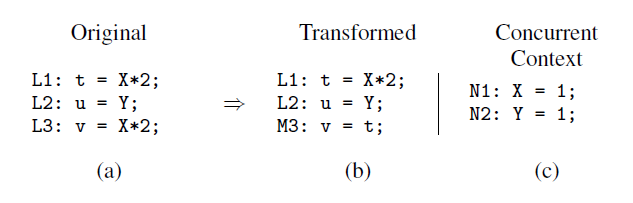
\includegraphics[scale=0.7]{NON-SC-TRANSF.PNG}
            }
        \end{figure}

    \end{frame}

    \notes{It is important to note that Common Sub-Expression Elimination is just one of the Non-SC preserving transformations.}

    %The view of Authors of the paper.
    \begin{frame}{A Counter view}

        The authors note in their empirical study of LLVM compiler optimization passes:
        \begin{itemize}
            \item Much of the performance in concurrent programs due to program transformations are already SC-Preserving. 
            \item A majority of Non-SC transformations responsible for much of the performance can be attributed to eager load/store transformations.
            \item These transformations can be summarized as reordering loads and stores throughout the program (thread-local).
            \item Part of these Non-SC transformations can be enabled using a simple speculation-based program constructs.  
        \end{itemize}
        
    \end{frame}

    \notes{It is important to note that many transformations rely on the primary assumption that they can freely reorder memory operations (eg:Register Alloaction, Constant Propagation, Scheduling, etc.).
    The fact that Reodering itself is Non-SC type indicates that a large class of transformations may be invalidated.
    I personally am unsure if the authors considered this as a fact during their empirical study.}

    \begin{frame}{List of Major SC-Preserving Transformations}

        %Attach the list here from paper.
        \begin{figure}
            \makebox[\textwidth][c]{
                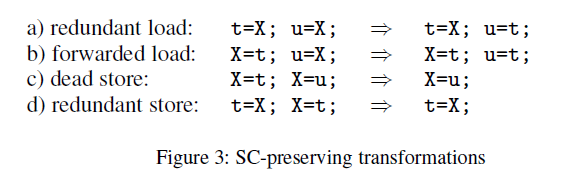
\includegraphics[scale=0.7]{SC-TRANSF.PNG}
            }
        \end{figure}

    \end{frame}

    \notes{Once again, we note that the above transformations are valid only standing alone.
    If they rely on reordering of memory operations, which in my experience is almost always, these transformations will be unsafe.}

    %Split reorderings in terms of relaxing L-L, L-S, S-L, S-S orders.
    \begin{frame}{Categorizing Reorderings}

        Reordering of memory accesses can be classified into four parts:
        \begin{itemize}
            \item Load-Load
            \item Load-Store
            \item Store-Load
            \item Store-Store
        \end{itemize}

        Such categories also are fences in certain hardware and software level memory models. 

        \begin{itemize}
            \item Allowing Eager load optimization is equivalent to eliminating Load-Load and Load-Store constraint.
            \item Allowing Eager store optimization is equivalent to elimination Store-Load and Store-Store constraint.
        \end{itemize}

    \end{frame}

    \notes{This way of classification is the exact dichotomy made by Doug Lea when describing the Java memory model.
    Different Hardwares also provide with fences that exactly mimic the syncrhonization barriers that prevents reordering of load-stores.}

    %Prime example where transformation will not be done as not SC-Preserving

    \begin{frame}{Example Being Optimized: SC-transformation}

        \begin{figure}
            \makebox[\textwidth][c]{
                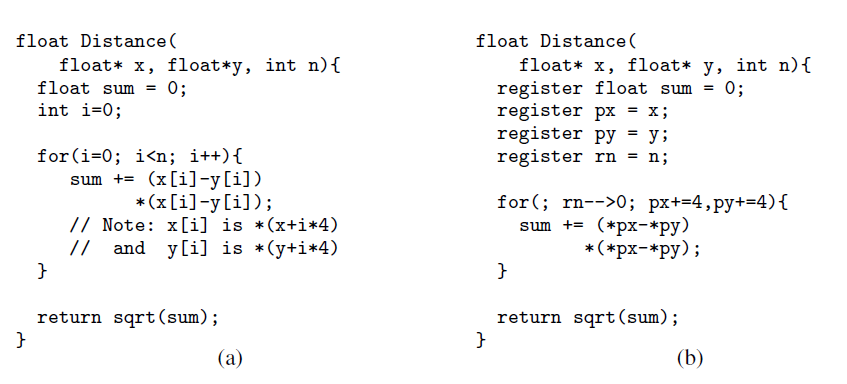
\includegraphics[scale=0.5]{TRANSF-EX-1.PNG}
            }
        \end{figure}
        
        %This will be a very involved example, so either explain by doodling here itself or find another way to explain.
    \end{frame}

    \begin{frame}{Example Being Optimized: Non-SC Transformation}

        \begin{figure}
            \makebox[\textwidth][c]{
                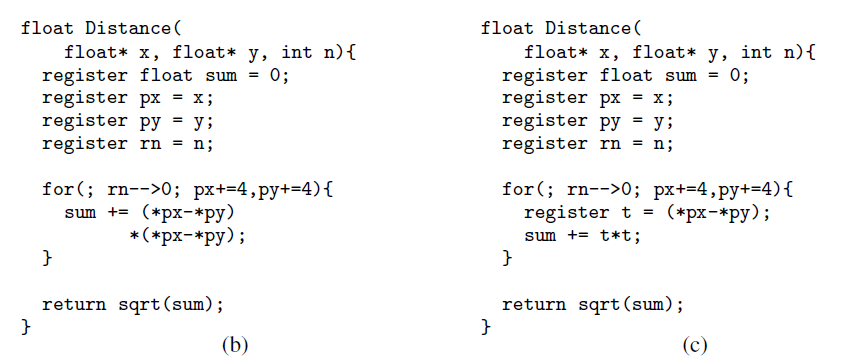
\includegraphics[scale=0.5]{TRANSF-EX-2.PNG}
            }
        \end{figure}
        
        %This will be a very involved example, so either explain by doodling here itself or find another way to explain.
    \end{frame}

    \notes{We can see that the non-SC transformation actually prevents two loads from memory of the same value. 
    However, note why it is not SC-Preserving: The second read to value at address of $y$ ($*py$), could imply a new value for the reads that were eliminated (due to for instance, Caches being invalidated or axiomatically, a new happens-before and coherence relation being generated).
    This would force us to have a non-SC behavior.}

    %Speculation idea in layman's terms 
    \begin{frame}{Idea of Speculation}

        \begin{itemize}
            \item Three base instructions. 
            \item Monitor load (\textit{m.load}).
            \item Monitor store (\textit{m.store}).
            \item Interference check (\textit{i.check}).
        \end{itemize}
        
    \end{frame}

    \notes{The main goal of using speculative style approach is to allow reorderings (eager loads and eager stores), which are generally non-SC, to be applied when there is no risk of relaxed behaviors in any execution.
    Monitor load/store for instance keeps a check on the memory on which they operate.
    Interference check is a boolean which indicates to us whether the specific monitored memory has been changed.
    If it did, then we cannot do eager load/store transformations.}

    \begin{frame}{Basic idea of Interference Check algorithm}
        
        \begin{figure}
            \makebox[\textwidth][c]{
                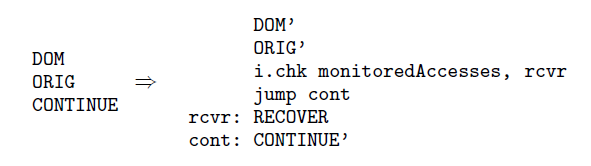
\includegraphics[scale=0.7]{INTERFERENCE-CHECK.PNG}
            }
        \end{figure}
        
    \end{frame}

    \notes{The algorithm sets the memory we want to perform eager load/store transformations to be mointored.
    If the memory values have changed beyond $ORIG'$, then just like speculation we run the $RECOVER$ block, else we run the $CONTINUE'$ block.}

    %Test-bed set up
    \begin{frame}{Evaluation strategy of performance}

        \begin{itemize}
            \item First no optimization.
            \item Then only SC-preserving.
            \item Then SC-Preserving with speculative checks.
            \item Then even non-SC opt.
        \end{itemize}
        
    \end{frame}

    
    \begin{frame}{Results}

        \begin{figure}
            \makebox[\textwidth][c]{
                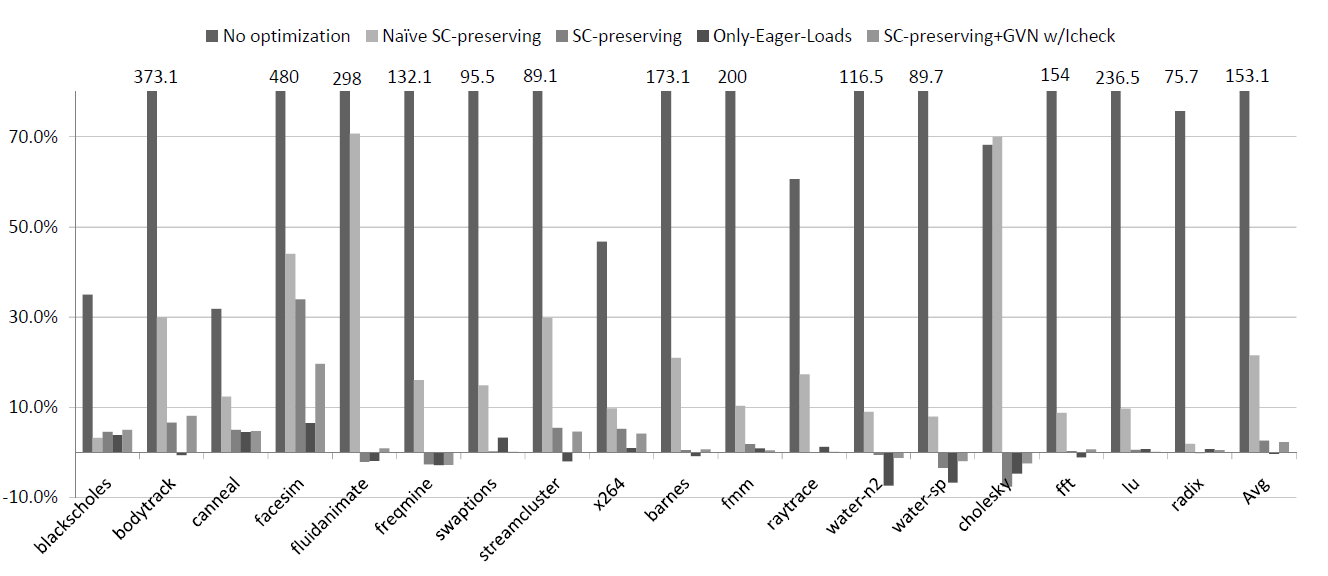
\includegraphics[scale=0.4]{EXPERIMENT-RESULTS.PNG}
            }
        \end{figure}

    \end{frame}

    \begin{frame}{Thank you}
        Questions?
    \end{frame}

\end{document}